\chapter{Árboles filogenéticos y reloj molecular}\label{ch:b2:phylogenetic-trees}

En 1965, dos químicos, Emile Zuckerkandl y Linus Pauling, compararon las
secuencias de aminoácidos de la hemoglobina de un puñado de vertebrados y
advirtieron algo que ningún anatomista habría podido ver: el número de
diferencias entre dos especies era proporcional al tiempo transcurrido
desde que sus antepasados se habían separado, tal como lo indicaban los
fósiles. Una molécula medía el tiempo. En menos de una década, Carl Woese
había usado un solo gen, el ARN de la subunidad pequeña del ribosoma, para
dibujar el árbol de toda la vida y encontrar en él un tercer dominio, las
arqueas, que ningún microscopio había distinguido de las bacterias. Este
capítulo trata de reconstruir la historia a partir del parecido: qué
significa un árbol, cómo se construye a partir de caracteres y de
distancias, cómo se hace que las secuencias den la hora, y las trampas ---
convergencia, tasas desiguales, saturación, ramas largas --- que debe
conocer quien lee árboles.

\section{Leer un árbol}

\begin{definition}[Filogenia, clado, homología]\label{def:b2:phylogenetic-trees:tree}
\index{filogenia}\index{clado}\index{grupo monofilético}\index{grupo parafilético}\index{grupo polifilético}\index{homología}\index{analogía}\index{sinapomorfía}
Una \emph{filogenia} es un árbol cuyas puntas son las especies (o los
genes, o los individuos) comparados, cuyos nodos internos son sus
antepasados comunes y cuya raíz es el antepasado más antiguo de todos. Solo
su orden de ramificación contiene la historia: los nodos pueden girarse
libremente, y solo importa el anidamiento. Un \emph{clado} o
\emph{grupo monofilético} es un antepasado con \emph{todos} sus
descendientes (las aves; los mamíferos; las aves y los cocodrilos juntos);
un grupo \emph{parafilético} es un antepasado al que se le han quitado
algunos descendientes (los ``reptiles'' sin las aves, los ``peces'' sin los
tetrápodos, los ``\omterm{def:b2:unicellular-diversity:prokaryote}{procariotas}''); un grupo \emph{polifilético} reúne
descendientes de antepasados distintos por un parecido que adquirieron por
separado (los ``animales de sangre caliente''). Un carácter compartido por
dos especies porque su antepasado lo tenía es una \emph{homología} (los
huesos del ala del murciélago y de la aleta de la ballena); uno que
adquirieron de forma independiente es una \emph{analogía} u
\emph{homoplasia} (las alas de los murciélagos y de las aves en cuanto
alas, los ojos en cámara de los vertebrados y de los pulpos). Solo las
homologías registran la historia, y entre ellas solo los estados
\emph{derivados} compartidos por un grupo --- sus
\emph{sinapomorfías}, el término de Hennig --- definen un clado: las
plumas definen a las aves; el estado ancestral ``sin plumas'' no define
nada.
\end{definition}
\begin{omfigure}
\begin{tikzpicture}[every node/.style={font=\scriptsize}, >=stealth, line width=0.8pt]
  \coordinate (root) at (0,0);
  \coordinate (n1) at (1.2,0.9); \coordinate (n2) at (2.4,1.6); \coordinate (n3) at (3.6,2.3);
  \draw (root) -- (1.4,-1.3) node[right] {mamíferos};
  \draw (root) -- (n1);
  \draw (n1) -- (4.8,-0.1) node[right] {tortugas};
  \draw (n1) -- (n2);
  \draw (n2) -- (4.8,0.9) node[right] {lagartos, serpientes};
  \draw (n2) -- (n3);
  \draw (n3) -- (4.8,1.9) node[right] {cocodrilos};
  \draw (n3) -- (4.8,3.0) node[right] {aves};
  \fill (root) circle (1.6pt); \fill (n1) circle (1.6pt); \fill (n2) circle (1.6pt); \fill (n3) circle (1.6pt);
  \node[left] at (root) {amniotas};
  % groups
  \draw[omThm, thick, rounded corners=6pt] (3.1,1.55) rectangle (6.9,3.4);
  \node[omThm, anchor=south west] at (3.1,3.4) {arcosaurios: monofilético};
  \draw[omExo!80!black, thick, dashed, rounded corners=6pt] (2.2,-0.5) -- (2.2,2.2) -- (7.1,2.2) -- (7.1,-0.5) -- cycle;
  \node[omExo!80!black, anchor=north east] at (7.1,-0.55) {``reptiles'' sin las aves: parafilético};
  \node[anchor=west, align=left, text width=4.2cm] at (7.9,1.3) {sinapomorfías:\\ $\bullet$ huevo amniótico (todos)\\ $\bullet$ abertura anteorbitaria en el cráneo (arcosaurios)\\ $\bullet$ plumas (aves)};
\end{tikzpicture}

{\small Leer un árbol. Las aves están anidadas dentro de los reptiles: los
cocodrilos están más próximos a las aves que a los lagartos. El grupo con
nombre ``reptiles'' es un antepasado al que se le ha quitado una línea de
descendientes --- un grado parafilético, no un \omterm{def:b2:phylogenetic-trees:tree}{clado}.}
\end{omfigure}

\begin{omfigure}
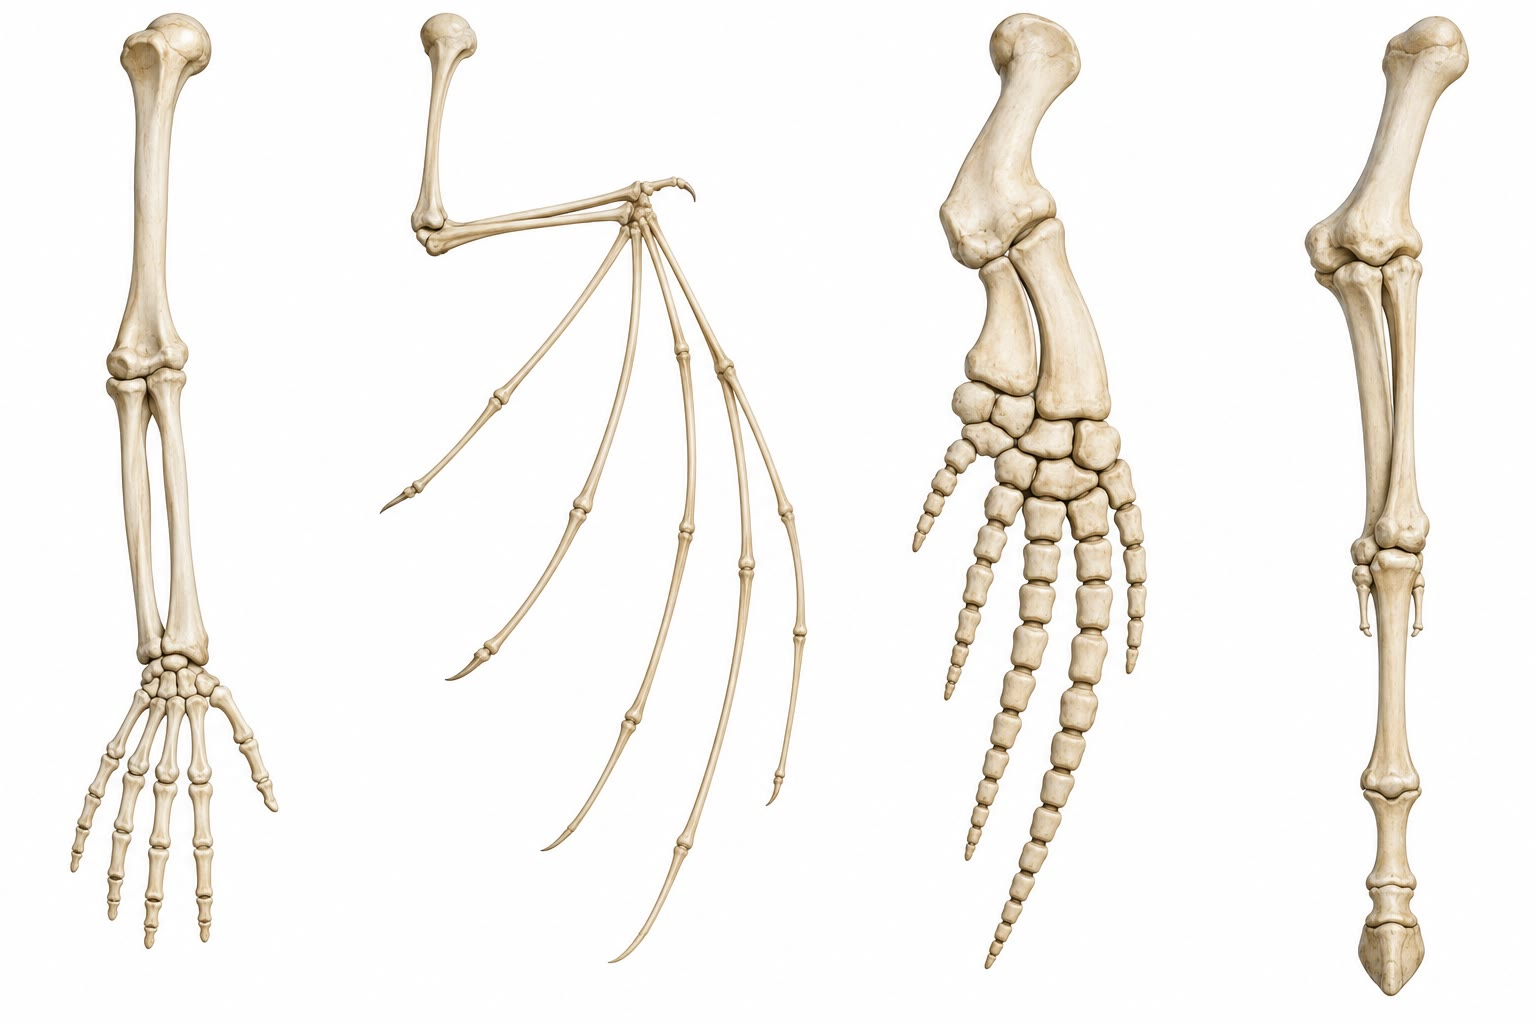
\includegraphics[width=0.44\linewidth]{images/book4/ai/b4-24-homologous-forelimbs.jpg}\hspace{0.04\linewidth}
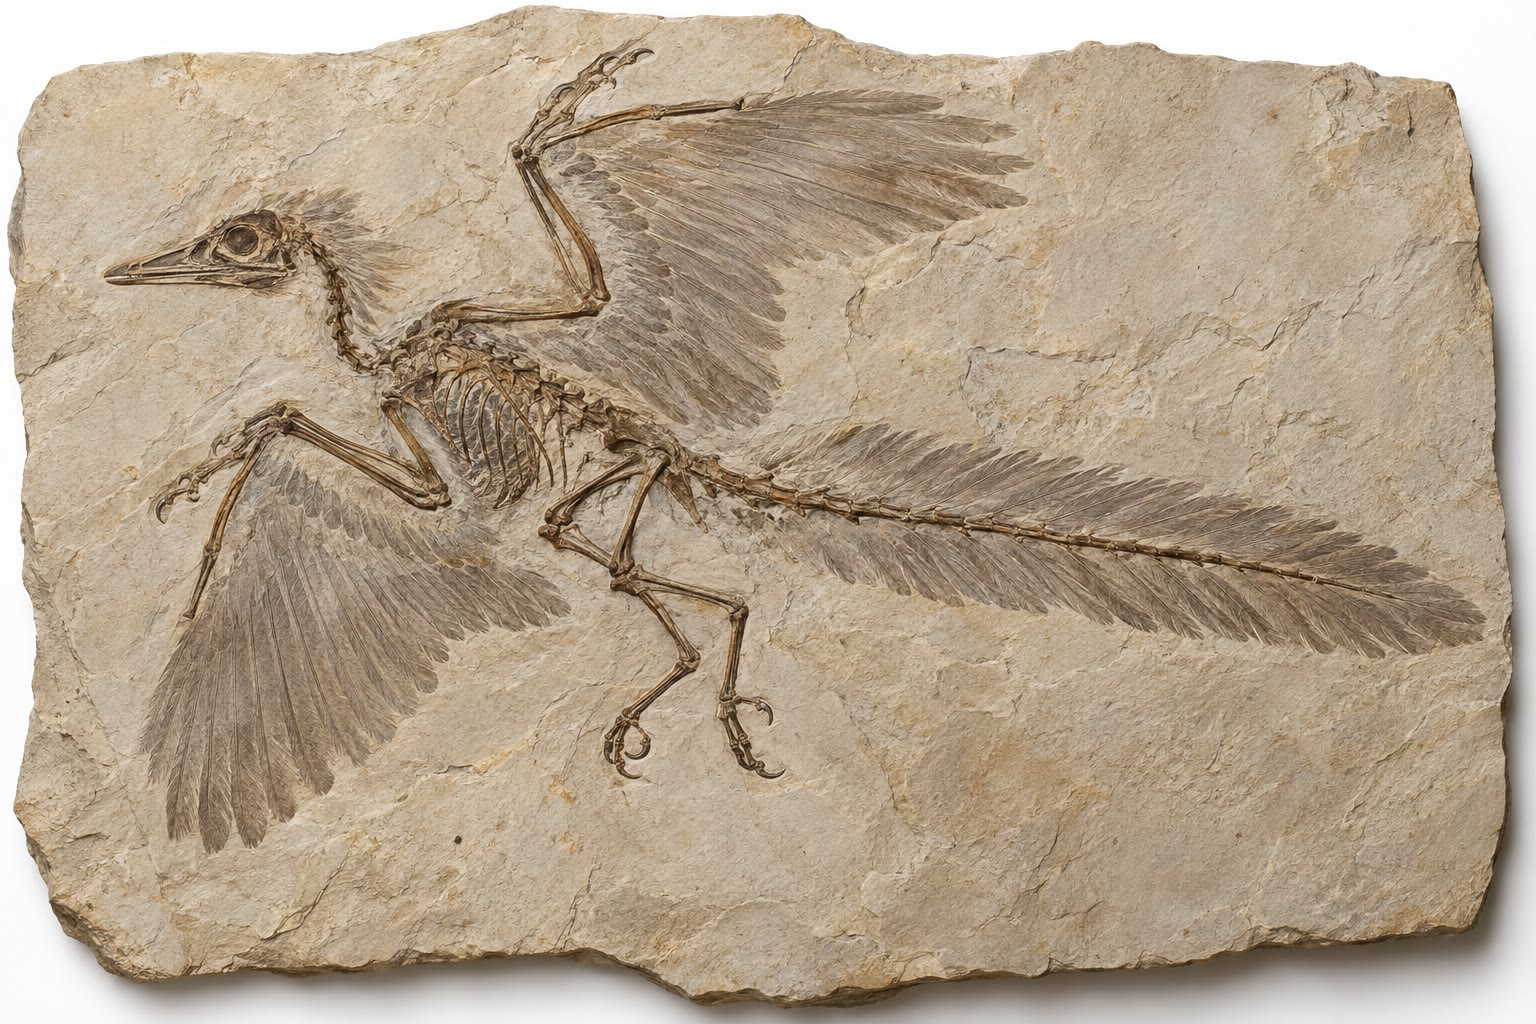
\includegraphics[width=0.44\linewidth]{images/book4/ai/b4-24-archaeopteryx.jpg}

{\small La \omterm{def:b2:phylogenetic-trees:tree}{homología} y su registro. Izquierda: los mismos huesos ---
húmero, radio y cúbito, muñeca, cinco dedos --- en un brazo, un ala, una
aleta y una pata. Derecha: \emph{Archaeopteryx}, con los dientes, los
dedos con garras y la larga cola ósea de un pequeño dinosaurio y las
plumas de un ave.}
\end{omfigure}

\section{Construir árboles a partir de caracteres}

\begin{method}[Parsimonia]\label{meth:b2:phylogenetic-trees:parsimony}
\index{parsimonia}\index{grupo externo}\index{bootstrap}
Se codifican los caracteres (estados morfológicos o posiciones de
secuencias alineadas) para cada taxón. Para cada árbol posible, se cuenta
el número mínimo de cambios de carácter necesarios para explicar los datos
sobre él; el árbol más parsimonioso es el que necesita menos. Se enraíza el
árbol con un \emph{\omterm{meth:b2:phylogenetic-trees:parsimony}{grupo externo}}, un taxón que se sabe situado fuera del
grupo estudiado. Como el número de árboles no enraizados para $n$ taxones
es $1\cdot 3\cdot
5\cdots(2n - 5)$ --- tres para cuatro taxones, $2\times 10^{6}$ para diez,
$10^{20}$ para veinte ---, la búsqueda solo es exhaustiva para conjuntos
pequeños y heurística más allá. La confianza se mide mediante el
\emph{bootstrap}: se remuestrean los caracteres con reposición mil veces,
se reconstruye el árbol cada vez y se registra con qué frecuencia reaparece
cada \omterm{def:b2:phylogenetic-trees:tree}{clado}; un \omterm{def:b2:phylogenetic-trees:tree}{clado} hallado en el \qty{95}{\%} de los remuestreos está
bien respaldado; uno hallado en la mitad, no.
\end{method}

\begin{example}[Cuatro taxones, cinco sitios]\label{ex:b2:phylogenetic-trees:parsimony}
Secuencias $A = \mathrm{AAGCT}$, $B = \mathrm{AAGCC}$, $C =
\mathrm{GGACT}$, $D = \mathrm{GGATC}$. Sobre el árbol $((A,B),(C,D))$,
los sitios 1, 2 y 3 cambian una vez cada uno (en la rama interna), el
sitio 4 una vez ($\mathrm{C}\to\mathrm{T}$ en $D$) y el sitio 5 dos veces
($\mathrm{T}\to\mathrm{C}$ en $B$ y en $D$): seis pasos. Sobre
$((A,C),(B,D))$, los sitios 1--3 necesitan dos cambios cada uno, y los
sitios 4 y 5, uno cada uno: ocho. Sobre $((A,D),(B,C))$: nueve. El primer
árbol es el más parsimonioso, por dos pasos; los tres sitios que lo
respaldan son sus \omterm{def:b2:phylogenetic-trees:tree}{sinapomorfías}, y el sitio 5 es una homoplasia sobre él
--- el mismo cambio ocurrido dos veces, algo habitual en cualquier conjunto
de datos real.
\end{example}

\begin{omfigure}
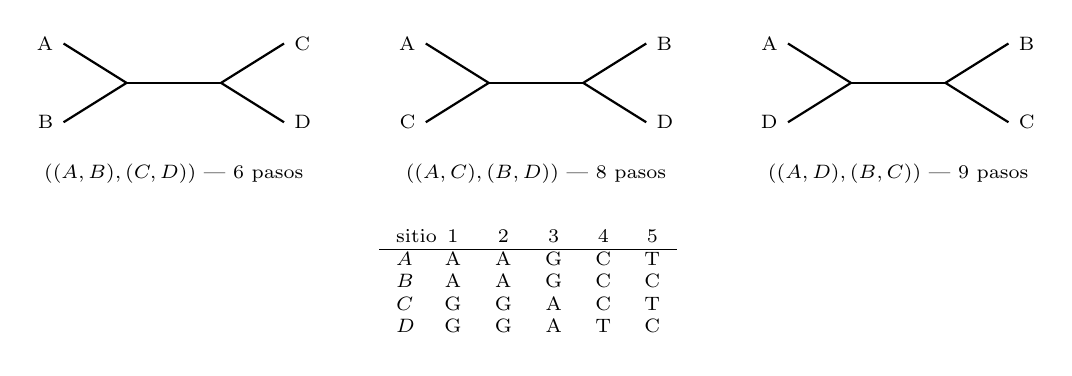
\begin{tikzpicture}[every node/.style={font=\scriptsize}, line width=0.8pt]
  \foreach \x/\a/\b/\c/\d/\steps/\lab in {0/A/B/C/D/6/{$((A,B),(C,D))$ --- 6 pasos}, 4.6/A/C/B/D/8/{$((A,C),(B,D))$ --- 8 pasos}, 9.2/A/D/B/C/9/{$((A,D),(B,C))$ --- 9 pasos}} {
    \begin{scope}[xshift=\x cm]
      \draw (0,1.6) node[left] {\a} -- (0.8,1.1) -- (0,0.6) node[left] {\b};
      \draw (0.8,1.1) -- (2.0,1.1);
      \draw (2.8,1.6) node[right] {\c} -- (2.0,1.1) -- (2.8,0.6) node[right] {\d};
      \node[anchor=north] at (1.4,0.2) {\lab};
    \end{scope}
  }
  \node[anchor=north] at (5.9,-0.6) {\begin{tabular}{l@{\ }ccccc} sitio & 1 & 2 & 3 & 4 & 5 \\ \hline $A$ & A & A & G & C & T \\ $B$ & A & A & G & C & C \\ $C$ & G & G & A & C & T \\ $D$ & G & G & A & T & C \end{tabular}};
\end{tikzpicture}

{\small Los tres árboles no enraizados para cuatro taxones, puntuados frente
al alineamiento de cinco sitios que figura debajo. Los sitios 1--3 cambian
una vez en el primer árbol y dos veces en los demás; el sitio 4 varía en un solo
taxón y no puede decidir, mientras que el sitio 5 agrupa $A$ con $C$ y
favorece por tanto el tercer árbol frente a ellos.}
\end{omfigure}

\section{Construir árboles a partir de distancias}

\begin{method}[Agrupamiento por distancias: UPGMA]\label{meth:b2:phylogenetic-trees:upgma}
\index{UPGMA}\index{unión de vecinos}\index{matriz de distancias}
A partir de las distancias por pares entre $n$ taxones (diferencias por
sitio, corregidas como se indica más abajo), se une el par más próximo en
un grupo situado en un nodo de altura igual a la mitad de su distancia; se
sustituye el par por el grupo, cuya distancia a cada uno de los demás
taxones es la media de las distancias de sus miembros; y se repite hasta
que queda un solo grupo. El resultado es un árbol enraizado con todas las
puntas a la misma altura --- supone una tasa de cambio constante en todas
las ramas, un \omterm{thm:b2:phylogenetic-trees:clock}{reloj molecular}. Cuando las tasas difieren entre linajes, el
método agrupa los linajes de evolución rápida sea cual sea su historia; la
\emph{\omterm{meth:b2:phylogenetic-trees:upgma}{unión de vecinos}},
que en cada paso une el par cuya unión acorta más el árbol entero, no
supone un reloj y es el método rápido estándar para grandes conjuntos de
datos.
\end{method}

\begin{example}[UPGMA]\label{ex:b2:phylogenetic-trees:upgma}
Distancias (en diferencias por cada cien sitios): $AB = 4$, $AC = 8$,
$AD = 10$, $BC = 8$, $BD = 10$, $CD = 6$. Se unen $A$ y $B$ a la altura 2;
entonces $d(AB, C) = 8$, $d(AB, D) = 10$, $d(C,D) = 6$: se unen $C$ y $D$
a la altura 3; por último, $d(AB, CD) = (8 + 10 + 8 + 10)/4 = 9$: se unen
los dos grupos a la altura $4.5$. El árbol es $((A,B),(C,D))$, y si
la tasa es de $10^{-9}$ sustituciones por sitio por año, la raíz tiene
$0.045/10^{-9} = 45$ millones de años.
\end{example}

\begin{omfigure}
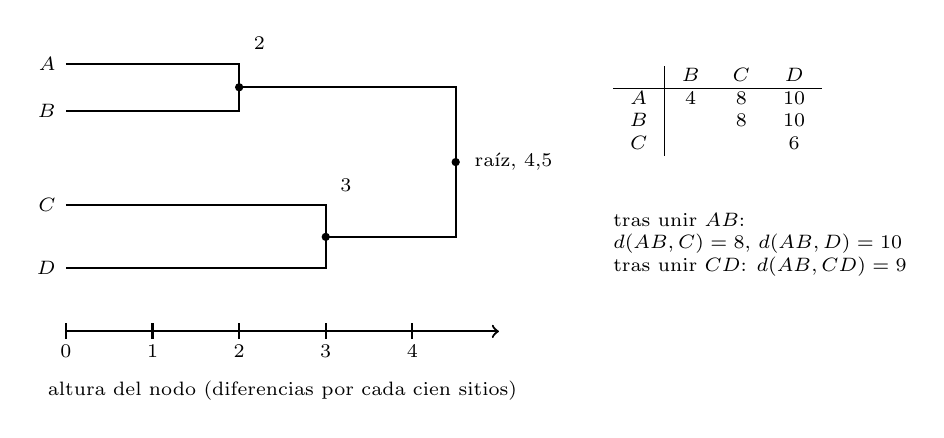
\begin{tikzpicture}[every node/.style={font=\scriptsize}, line width=0.8pt, x=1.1cm]
  \draw[->] (0,-0.4) -- (5,-0.4); \foreach \h in {0,1,2,3,4} \draw (\h,-0.5) -- (\h,-0.3) node[below=4pt] {\h};
  \node[anchor=north] at (2.5,-0.9) {altura del nodo (diferencias por cada cien sitios)};
  % A,B join at 2, C,D at 3, root at 4.5 ; draw as rooted tree, root on the right
  \draw (0,3.0) node[left] {$A$} -- (2,3.0) -- (2,2.4) -- (0,2.4) node[left] {$B$};
  \draw (0,1.2) node[left] {$C$} -- (3,1.2) -- (3,0.4) -- (0,0.4) node[left] {$D$};
  \draw (2,2.7) -- (4.5,2.7) -- (4.5,0.8) -- (3,0.8);
  \fill (2,2.7) circle (1.5pt); \fill (3,0.8) circle (1.5pt); \fill (4.5,1.75) circle (1.5pt);
  \node[anchor=west] at (4.6,1.75) {raíz, 4,5};
  \node[anchor=south west] at (2.05,3.05) {2};
  \node[anchor=south west] at (3.05,1.25) {3};
  \node[anchor=west, align=left] at (6.2,2.4) {\begin{tabular}{c|ccc} & $B$ & $C$ & $D$ \\ \hline $A$ & 4 & 8 & 10 \\ $B$ & & 8 & 10 \\ $C$ & & & 6 \end{tabular}};
  \node[anchor=west, align=left] at (6.2,0.7) {tras unir $AB$:\\ $d(AB,C) = 8$, $d(AB,D) = 10$\\ tras unir $CD$: $d(AB,CD) = 9$};
\end{tikzpicture}

{\small UPGMA sobre cuatro taxones. Cada nodo se sitúa a la mitad de la
distancia entre los grupos que une; todas las puntas terminan a la altura
cero, como exige un reloj.}
\end{omfigure}

\section{El reloj molecular}

\begin{theorem}[Las sustituciones como proceso de Poisson, y la corrección de los impactos múltiples]\label{thm:b2:phylogenetic-trees:clock}
\index{reloj molecular}\index{corrección de Jukes--Cantor}\index{saturación}
Si las sustituciones en un sitio se producen a una tasa constante $k$ por
año, con independencia entre sitios, el número que se acumula a lo largo
de un linaje en un tiempo $t$ sigue una ley de Poisson de media $kt$, y el
número esperado que separa dos linajes que divergieron hace $t$ años es
\[
d = 2kt
\]
sustituciones por sitio --- el \emph{\omterm{thm:b2:phylogenetic-trees:clock}{reloj molecular}}. La proporción
observada $p$ de sitios que difieren es menor que $d$, porque un sitio
alcanzado dos veces puede volver a su base original o coincidir por azar;
con cuatro bases que cambian a tasas iguales,
\[
p = \tfrac{3}{4}\bigl(1 - e^{-4d/3}\bigr), \qquad
d = -\tfrac{3}{4}\ln\bigl(1 - \tfrac{4}{3}p\bigr),
\]
la corrección de \emph{Jukes--Cantor}. A medida que crece $d$, $p$ se
satura en
$3/4$ --- dos secuencias aleatorias coinciden en una cuarta parte de sus
sitios --- y más allá de $p \approx 0.5$ la corrección amplifica cualquier
error de muestreo: un gen que ha cambiado tanto ha dejado de medir el
tiempo. Los genes lentos (ARN ribosómico, histonas) datan las ramas
profundas; los rápidos (ADN mitocondrial, intrones), las recientes.
\end{theorem}
\begin{proof}
Sea $q(t)$ la probabilidad de que un sitio conserve todavía su base
original al cabo de un tiempo $t$. La pierde a una tasa $k$ y la recupera,
a partir de cualquiera de las otras tres bases, a una tasa $k/3$:
$\mathrm{d}q/\mathrm{d}t = -kq + \tfrac{k}{3}(1 - q) = \tfrac{k}{3} -
\tfrac{4k}{3}q$, cuya solución con $q(0) = 1$ es $q = \tfrac14 +
\tfrac34 e^{-4kt/3}$. Dos linajes separados por un tiempo total $2t$ ---
por simetría, lo mismo que un solo linaje que evoluciona durante $2t$ ---
coinciden en un sitio con probabilidad $\tfrac14 + \tfrac34 e^{-4d/3}$, donde $d =
2kt$, de modo que $p = 1 - q = \tfrac34(1 - e^{-4d/3})$; invirtiendo se
obtiene la corrección. El recuento de Poisson se deduce de sucesos
constantes e independientes, como en la física de la desintegración
radiactiva, y su desviación típica $\sqrt{kt}$ fija la precisión de
cualquier fecha: un gen de $L$
sitios con $dL$ sustituciones observadas data una divergencia con una
precisión relativa de alrededor de $1/\sqrt{dL}$.
\end{proof}
\begin{proof}[Evidencia]
Zuckerkandl y Pauling (1965) hallaron que las diferencias entre las
hemoglobinas del caballo, el ser humano, la vaca y otras especies eran
proporcionales a las edades fósiles de sus separaciones, y propusieron el
reloj. Fitch y Margoliash (1967) construyeron un árbol de veinte especies
solo a partir del citocromo
$c$ y recuperaron, con una sola proteína, las agrupaciones clásicas de
vertebrados, insectos y hongos. La prueba decisiva del método fue la
\omterm{def:b2:phylogenetic-trees:tree}{filogenia} experimental de Hillis y sus colaboradores (1992): propagaron el
bacteriófago T7 a lo largo de una serie ramificada y conocida de ocho
linajes en presencia de un mutágeno, secuenciaron los productos y dieron
las secuencias a ciegas a los métodos de construcción de árboles ---
los métodos de parsimonia, de distancias y de verosimilitud recuperaron
todos el árbol verdadero, y la parsimonia reconstruyó las secuencias
ancestrales con una exactitud superior al
\qty{98}{\%}.
\end{proof}

\begin{omfigure}
\begin{tikzpicture}
\begin{axis}[
  width=0.7\linewidth, height=5.4cm,
  axis x line=bottom, axis y line=left,
  xmin=0, xmax=2.5, ymin=0, ymax=1.05,
  xlabel={sustituciones reales por sitio, $d$}, ylabel={diferencias observadas, $p$},
  xlabel style={font=\small, at={(axis description cs:0.5,-0.13)}, anchor=north},
  ylabel style={font=\small},
  tick label style={font=\small}, ytick={0,0.25,0.5,0.75,1},
  legend style={font=\scriptsize, at={(0.97,0.35)}, anchor=east, draw=none},
  clip=false,
]
\addplot[very thick, omDef, domain=0:2.5, samples=80] {0.75*(1-exp(-4*x/3))};
\addlegendentry{$p = \tfrac34(1 - e^{-4d/3})$}
\addplot[thick, gray, dashed, domain=0:1.05, samples=2] {x};
\addlegendentry{$p = d$: sin impactos múltiples}
\draw[dotted, gray] (axis cs:0,0.75) -- (axis cs:2.5,0.75); \node[font=\scriptsize, anchor=south east] at (axis cs:2.5,0.75) {saturación, $p = 3/4$};
\draw[<->, omThm, thick] (axis cs:0.383,0.30) -- (axis cs:0.383,0.383); \node[font=\scriptsize, omThm, anchor=west] at (axis cs:0.5,0.22) {$p = 0.30$ significa $d = 0.38$};
\end{axis}
\end{tikzpicture}

{\small Impactos múltiples. La fracción observada de sitios que difieren
aumenta con el número real de sustituciones y después se satura; una $p$
sin corregir subestima todas las distancias y comprime las ramas profundas
de un árbol.}
\end{omfigure}

\begin{proposition}[Las trampas del reloj y de los árboles]\label{prop:b2:phylogenetic-trees:pitfalls}
\index{atracción de ramas largas}\index{heterogeneidad de tasas}\index{separación incompleta de linajes}\index{verosimilitud (filogenética)}
El reloj solo es aproximadamente constante: las tasas difieren entre genes
en un factor cien (según la función --- la histona H4 ha cambiado dos
residuos en mil millones de años, los fibrinopéptidos cambian cada pocos
millones), entre sitios dentro de un gen (las terceras posiciones de los
codones, los intrones y los bucles cambian más deprisa) y entre linajes
(los roedores avanzan más deprisa que los primates, con sus generaciones
más cortas y sus tasas metabólicas más altas). Todo reloj necesita, por
tanto, una \emph{calibración} mediante un fósil o un acontecimiento
geológico datado, y las fechas llevan el error de Poisson citado y el de la
propia calibración. Los árboles tienen sus propias trampas. La
\emph{\omterm{prop:b2:phylogenetic-trees:pitfalls}{atracción de ramas largas}}: dos linajes que han cambiado mucho cada
uno comparten muchos sitios por azar, y la parsimonia los une sea cual sea
su historia --- el remedio es un muestreo más denso para romper las ramas y
un método que modelice las tasas. La \emph{convergencia} produce falsas
\omterm{def:b2:phylogenetic-trees:tree}{sinapomorfías}. La
\emph{\omterm{prop:b2:phylogenetic-trees:pitfalls}{separación incompleta de linajes}}: el árbol de un gen no tiene por
qué ser el de las especies cuando las especiaciones se suceden deprisa,
porque el polimorfismo ancestral se reparte de forma distinta en cada
descendiente --- por eso un árbol de especies se construye con muchos genes,
no con uno. Y en los \omterm{def:b2:unicellular-diversity:prokaryote}{procariotas}, donde los genes se desplazan
lateralmente (\cref{ch:b2:genome-diversification}), genes distintos
cuentan historias distintas y la historia es una red atravesada por un
árbol de genes ribosómicos. La práctica moderna sustituye la parsimonia y
las distancias por la \emph{verosimilitud}: dado un modelo de sustitución
(las tasas de cada cambio, su variación entre sitios), se calcula la
probabilidad de las secuencias observadas sobre cada árbol con sus
longitudes de rama y se elige el árbol que hace más probables los datos;
su forma bayesiana da directamente una probabilidad para cada \omterm{def:b2:phylogenetic-trees:tree}{clado}. El
volumen del tercer año presenta los métodos; aquí basta con saber que
todo árbol es una hipótesis con un respaldo medido, no un hecho.
\end{proposition}
\begin{proof}[Evidencia]
Woese y Fox (1977) compararon el ARN ribosómico de la subunidad pequeña en
distintos \omterm{def:b2:unicellular-diversity:prokaryote}{procariotas} y hallaron que los metanógenos estaban tan alejados
de las bacterias como cualquiera de ambos grupos lo está de los eucariotas:
los tres dominios, confirmados desde entonces por todos los genes de la
maquinaria de transcripción y traducción, e invisibles para la morfología.
Esos mismos árboles ribosómicos, leídos ingenuamente, situaban los
microsporidios, de evolución rápida, en la base de los eucariotas; los
genes de tasas más lentas y los modelos que tienen en cuenta la variación
de las tasas los desplazaron a los hongos, donde les corresponde --- un
caso de manual de \omterm{prop:b2:phylogenetic-trees:pitfalls}{atracción de ramas largas} detectada y corregida.
\end{proof}

\begin{omfigure}
\begin{tikzpicture}[every node/.style={font=\scriptsize}, line width=0.8pt]
  \node[anchor=south] at (1.5,2.6) {árbol verdadero};
  \draw (0,2.2) node[left] {$A$} -- (0.8,1.6) -- (0,1.0) node[left] {$B$};
  \draw (0.8,1.6) -- (1.6,1.6);
  \draw[very thick, omThm] (1.6,1.6) -- (3.4,2.4) node[right] {$C$ (rápido)};
  \draw[very thick, omThm] (0.8,1.6) -- (0.8,0.2) -- (2.6,0.2) node[right] {$D$ (rápido)};
  \draw (1.6,1.6) -- (2.4,1.0) node[right] {$E$};
  \begin{scope}[xshift=7cm]
    \node[anchor=south] at (1.5,2.6) {árbol que halla la parsimonia};
    \draw (0,2.2) node[left] {$A$} -- (0.8,1.6) -- (0,1.0) node[left] {$B$};
    \draw (0.8,1.6) -- (1.6,1.6);
    \draw (1.6,1.6) -- (2.4,1.9) node[right] {$E$};
    \draw[very thick, omThm] (1.6,1.6) -- (2.2,1.0) -- (3.4,1.3) node[right] {$C$};
    \draw[very thick, omThm] (2.2,1.0) -- (3.0,0.2) node[right] {$D$};
  \end{scope}
  \node[align=center, text width=7cm] at (5.6,-1.1) {$C$ y $D$ han cambiado cada uno en muchos sitios; en una cuarta parte de ellos coinciden ahora por azar, más de lo que cualquier sinapomorfía verdadera los une a sus parientes reales};
\end{tikzpicture}

{\small \omterm{prop:b2:phylogenetic-trees:pitfalls}{Atracción de ramas largas}. Dos linajes que han evolucionado más
deprisa quedan unidos por las coincidencias fortuitas que producen sus
numerosos cambios, y la parsimonia los convierte en grupos hermanos.}
\end{omfigure}

\begin{example}[Datar con un fósil]\label{ex:b2:phylogenetic-trees:dating}
Un gen de \num{1000} sitios difiere en el \qty{10}{\%} de ellos entre la
vaca y la ballena, cuyo antepasado común sitúan los fósiles hace 60
millones de años. Corregida, $d = -0.75\ln(1 - 0.133) = 0.107$; la tasa es $k
= d/2t = 0.107/(1.2\times 10^{8}) = 9\times 10^{-10}$ por sitio por
año. El mismo gen difiere en el \qty{6}{\%} entre la ballena y el
hipopótamo: $d = 0.0625$, $t = d/2k = 35$ millones de años, con alrededor
de un $\pm
\qty{13}{\%}$ debido al recuento de Poisson de 62 sustituciones y una
incertidumbre adicional debida a la fecha del fósil. El resultado
molecular de que las ballenas son los parientes vivos más próximos de los
hipopótamos, obtenido así en la década de 1990 en contra de todos los
árboles anatómicos, lo confirmó el descubrimiento de ballenas primitivas
con el astrágalo de tipo hipopótamo que se había predicho --- el reloj no
solo data; predice lo que deben contener las rocas.
\end{example}

\section{Ejercicios}

\begin{exercise}[$\star$]\label{exo:b2:phylogenetic-trees:1}
Defínanse \omterm{def:b2:phylogenetic-trees:tree}{homología}, \omterm{def:b2:phylogenetic-trees:tree}{analogía} y \omterm{def:b2:phylogenetic-trees:tree}{sinapomorfía}, con un ejemplo de cada una
entre los miembros, las alas y los ojos de los vertebrados.
\end{exercise}

\begin{exercise}[$\star$]\label{exo:b2:phylogenetic-trees:2}
Clasifíquense como monofiléticos, parafiléticos o polifiléticos: las aves;
los reptiles (sin las aves); los peces (sin los tetrápodos); los
vertebrados voladores; los mamíferos; los \omterm{def:b2:unicellular-diversity:prokaryote}{procariotas}.
\end{exercise}

\begin{exercise}[$\star$]\label{exo:b2:phylogenetic-trees:3}
Sobre el árbol $(\text{mamíferos},(\text{tortugas},(\text{lagartos},
(\text{cocodrilos},\text{aves}))))$, nómbrense el grupo hermano de las
aves, el grupo hermano de los mamíferos y el \omterm{def:b2:phylogenetic-trees:tree}{clado} más pequeño que
contiene a los lagartos y a las aves. ¿Cambia el árbol si se intercambian
las posiciones de los cocodrilos y las aves?
\end{exercise}

\begin{exercise}[$\star$]\label{exo:b2:phylogenetic-trees:4}
¿Cuántos árboles no enraizados hay para 4, 6 y 10 taxones? ¿Cuántos
árboles enraizados para 4 (cada árbol no enraizado puede enraizarse en
cualquiera de sus ramas)?
\end{exercise}

\begin{exercise}[$\star\star$]\label{exo:b2:phylogenetic-trees:5}
Secuencias $A = \mathrm{CCTAG}$, $B = \mathrm{CCTGG}$, $C =
\mathrm{TTCAG}$, $D = \mathrm{TTCGA}$. Cuéntense los pasos en cada uno de
los tres árboles no enraizados e indíquese el más parsimonioso. ¿Qué
sitios son homoplásicos en él?
\end{exercise}

\begin{exercise}[$\star\star$]\label{exo:b2:phylogenetic-trees:6}
Distancias (por cada cien sitios): $AB = 6$, $AC = 14$, $AD = 16$,
$BC = 14$, $BD = 16$, $CD = 10$. Constrúyase el árbol UPGMA con las
alturas de sus nodos.
\end{exercise}

\begin{exercise}[$\star\star$]\label{exo:b2:phylogenetic-trees:7}
Corríjanse $p = 0.05$, $0.30$ y $0.60$ para los impactos múltiples. ¿Por
qué el tercer valor es casi inútil?
\end{exercise}

\begin{exercise}[$\star\star$]\label{exo:b2:phylogenetic-trees:8}
Un gen evoluciona a $10^{-9}$ sustituciones por sitio por año. Dos
especies difieren en $d = 0.02$: ¿cuándo se separaron? ¿Qué $p$ se
observaría entre dos especies que se separaron hace 500 millones de años,
y qué implica eso para datar separaciones profundas con este gen?
\end{exercise}

\begin{exercise}[$\star\star$]\label{exo:b2:phylogenetic-trees:9}
Un \omterm{def:b2:phylogenetic-trees:tree}{clado} aparece en el \qty{52}{\%} de \num{1000} remuestreos bootstrap;
otro, en el \qty{99}{\%}. Interprétense ambos. ¿Qué habría que hacer con el
primero?
\end{exercise}

\begin{exercise}[$\star\star\star$]\label{exo:b2:phylogenetic-trees:10}
Explíquese la \omterm{prop:b2:phylogenetic-trees:pitfalls}{atracción de ramas largas} con el argumento de la cuarta
parte por azar, e indíquese por qué ayuda añadir taxones que rompan las
ramas largas.
\end{exercise}

\begin{exercise}[$\star\star\star$]\label{exo:b2:phylogenetic-trees:11}
El ADN mitocondrial del ser humano y el del chimpancé difieren en el
\qty{9}{\%} de los sitios; la tasa mitocondrial es de alrededor de
$2\times 10^{-8}$ por sitio por año. Dátese la separación, dese la
incertidumbre de Poisson para un genoma de \qty{16000}{} sitios y
nómbrense dos razones por las que el resultado podría seguir siendo
erróneo en un factor dos.
\end{exercise}

\begin{exercise}[$\star\star\star$]\label{exo:b2:phylogenetic-trees:12}
``Un árbol de genes no es un árbol de especies.'' Discútase con la
\omterm{prop:b2:phylogenetic-trees:pitfalls}{separación incompleta de linajes}, la transferencia horizontal y la
\omterm{prop:b2:genome-diversification:duplication}{duplicación génica}, e indíquese cómo se obtiene, pese a todo, un árbol de
especies.
\end{exercise}

\section{Problema: datar las ballenas}

\begin{problem}[{Problema de fin de semana --- ballena, hipopótamo, vaca,
cerdo y camello secuenciados para un gen: el árbol construido por
parsimonia y por distancias, el reloj calibrado con un fósil, cada
separación datada con su error de Poisson y el árbol anatómico confrontado
con el molecular, hasta llegar al tiempo de divergencia entre ballena e
hipopótamo y a la tasa de sustitución del gen}]
\label{pb:b2:phylogenetic-trees:1}
Se secuencia un gen de \num{1000} sitios en la ballena ($W$), el
hipopótamo ($H$), la vaca ($C$), el cerdo ($P$) y el camello ($M$, el
\omterm{meth:b2:phylogenetic-trees:parsimony}{grupo externo}). Proporciones observadas de sitios que difieren: $WH = 0.06$; $WC = HC = 0.10$; $WP =
HP = CP = 0.12$; todas las distancias a $M$ valen $0.14$. Los fósiles
sitúan la separación entre la vaca y la línea ballena--hipopótamo hace 60
millones de años. Seis sitios informativos, con el estado del camello en
último lugar:
\begin{center}
\begin{tabular}{l@{\quad}cccccc}
sitio & 1 & 2 & 3 & 4 & 5 & 6 \\ \hline
$W$ & A & G & T & C & A & G \\
$H$ & A & G & T & C & G & G \\
$C$ & G & A & T & T & G & G \\
$P$ & G & A & C & T & G & A \\
$M$ & G & A & C & T & G & A \\
\end{tabular}
\end{center}

\medskip
\noindent\textbf{Parte I --- Parsimonia.}
\begin{enumerate}
  \item ¿Qué sitios son \omterm{def:b2:phylogenetic-trees:tree}{sinapomorfías} de $\{W, H\}$? ¿Y de $\{W, H,
        C\}$? ¿Qué sitio no es informativo, y cuál es una homoplasia
        o una autapomorfía?
  \item Cuéntense los pasos de los seis sitios sobre el árbol
        $(M,(P,(C,(W,H))))$.
  \item Cuéntense sobre el árbol de los anatomistas, $(M,(P,(W,(C,H))))$,
        que sitúa al hipopótamo con la vaca entre los ungulados de dedos
        pares y a las ballenas fuera.
  \item ¿Qué árbol se prefiere, y por cuántos pasos? ¿Por qué es débil ese
        margen, y qué lo reforzaría?
  \item El bootstrap da el \omterm{def:b2:phylogenetic-trees:tree}{clado} $\{W, H\}$ en el \qty{83}{\%} de los
        remuestreos del gen completo. Interprétese.
  \item ¿Por qué se usa el camello como \omterm{meth:b2:phylogenetic-trees:parsimony}{grupo externo}, y qué fallaría si se
        usara un pez?
\end{enumerate}

\medskip
\noindent\textbf{Parte II --- Distancias.}
\begin{enumerate}[resume]
  \item Corríjanse los cuatro valores distintos de $p$ ($0.06$, $0.10$, $0.12$,
        $0.14$) para los impactos múltiples.
  \item Aplíquese el UPGMA a los cinco taxones con las distancias
        corregidas y dense las alturas de los nodos.
  \item ¿Coincide el árbol de distancias con el de parsimonia?
  \item Explíquese por qué fallaría el UPGMA si el linaje de la ballena
        hubiera evolucionado el doble de deprisa que los demás.
  \item Calcúlense el número de sustituciones que ha acumulado el gen entre
        la ballena y el hipopótamo, y su desviación típica de Poisson.
  \item Dese la precisión relativa de una fecha basada en ese recuento.
\end{enumerate}

\medskip
\noindent\textbf{Parte III --- El reloj.}
\begin{enumerate}[resume]
  \item Calíbrese: a partir de la distancia entre la vaca y el par
        (ballena, hipopótamo) y del fósil de 60 millones de años,
        calcúlese la tasa $k$ por sitio por año.
  \item Dátese la separación entre ballena e hipopótamo.
  \item Dátense la separación del cerdo y la del camello.
  \item Dese la fecha de la separación entre ballena e hipopótamo con su
        incertidumbre de Poisson.
  \item La calibración fósil tiene a su vez una incertidumbre de $\pm 5$
        millones de años. Propáguese a la fecha de la separación entre
        ballena e hipopótamo.
  \item Otro gen, más rápido, da $p = 0.45$ entre la ballena y el camello.
        Corríjase y coméntese su fiabilidad para esta separación.
\end{enumerate}

\medskip
\noindent\textbf{Parte IV --- Confrontación.}
\begin{enumerate}[resume]
  \item El árbol de los anatomistas se basa en el astrágalo de doble polea
        que comparten la vaca, el cerdo, el hipopótamo y el camello, pero
        no las ballenas actuales, que no tienen patas traseras. Explíquese
        por qué un carácter perdido no puede contar en contra del \omterm{def:b2:phylogenetic-trees:tree}{clado}
        ballena--hipopótamo.
  \item En 2001 se hallaron ballenas fósiles con patas traseras; su
        astrágalo tiene la doble polea. ¿Qué efecto tiene eso sobre el
        argumento?
  \item Si las ballenas están dentro de los ungulados de dedos pares, ¿es
        el grupo ``ungulados de dedos pares sin las ballenas'' monofilético,
        parafilético o polifilético?
  \item Un segundo gen da el árbol $(M,(P,(H,(W,C))))$. Nómbrense dos
        razones por las que un árbol de genes puede diferir del árbol de
        especies, e indíquese cómo decidir.
  \item El genoma mitocondrial de la ballena y el del hipopótamo difieren
        en el \qty{25}{\%} de los sitios. Corríjase y estímese la tasa
        mitocondrial a partir de la fecha hallada en la pregunta 14.
  \item ¿Por qué esa tasa es tan superior a la del gen nuclear?
  \item Enúnciese el resultado: el árbol, la tasa nuclear $k$ y el tiempo
        de divergencia entre ballena e hipopótamo con su incertidumbre.
\end{enumerate}
\end{problem}
